\documentclass[../../main.tex]{subfiles}
\graphicspath{{\subfix{../images/}}} % 指定图片目录,后续可以直接使用图片文件名。
\begin{document}
\section{Homework 4}
\subsection{Van der Waals equation}
  \begin{enumerate}
    \item \textbf{Derive for the dimensionless van der Waals equation of state from the original vdW equation $\begin{aligned}
      P = \frac{RT}{v-b} - \frac{a}{v^{2}}
    \end{aligned}$.} 

    The conditions for the critical point are
    \begin{align*}
      \left(\frac{\partial P}{\partial v}\right)_{T} = 0,\quad \left(\frac{\partial^{2} P}{\partial v^{2}}\right)_{T} = 0.
    \end{align*}
    So compute the derivatives of the pressure $P$:
    \begin{align*}
      \begin{cases}
        \frac{\partial P}{\partial v} &= -\frac{RT}{(v-b)^{2}} + \frac{2a}{v^{3}},\\
      \frac{\partial^{2}P}{\partial v^{2}} &= \frac{2RT}{(v-b)^{3}} - \frac{6a}{v^{4}}.
      \end{cases}
    \end{align*}
    At the critical point, let $v = v_{c}$, $P = P_{c}$, $T = T_{c}$, and we have the following equations:
    \begin{align*}
      \begin{cases}
        \frac{RT_{c}}{(v_{c}-b)^{2}} - \frac{2a}{v_{c}^{3}} &= 0,\\
        \frac{2RT_{c}}{(v_{c}-b)^{3}} - \frac{6a}{v_{c}^{4}} &= 0.
      \end{cases}
      \Rightarrow \begin{cases}
        RT_{c} &= \frac{2a(v_{c}-b)^{2}}{v_{c}^{3}},\\
        RT_{c} &= \frac{3a(v_{c}-b)^{3}}{v_{c}^{4}}.
      \end{cases}
      \Rightarrow v_{c} = 3b
    \end{align*}
    Since $v_{c}$ has been determined, we can substitute it into the first equation to get:
    \begin{align*}
      RT_{c} &= \frac{2a(3b-b)^{2}}{(3b)^{3}} = \frac{8a}{27b}\Rightarrow T_{c} = \frac{8a}{27Rb}\\
      P_{c} &= \frac{RT_{c}}{v_{c}-b} - \frac{a}{v_{c}^{2}} = \frac{a}{27b^{2}}.
    \end{align*}
    Rescale the variables with the critical conditions:
    \begin{align*}
      P_{r} &= \frac{P}{P_{c}},\quad v_{r} = \frac{v}{v_{c}},\quad T_{r} = \frac{T}{T_{c}}.\\
      \Leftrightarrow P &= P_{r}P_{c} = P_{r}\cdot\frac{a}{27b^{2}},\quad v = v_{r}v_{c} = v_{r}\cdot 3b,\quad T = T_{r}T_{c} = T_{r}\cdot\frac{8a}{27Rb}.
    \end{align*}
    So the van der Waals equation of state come to be
    \begin{align*}
      P_{r}\cdot \frac{a}{27b^{2}} = \frac{RT_{r}\cdot\frac{8a}{27Rb}}{v_{r}\cdot 3b - b} - \frac{a}{(v_{r}\cdot 3b)^{2}}\\
      \Rightarrow P_{r} = \frac{8T_{r}}{3v_{r}-1} - \frac{3}{v_{r}^{2}}.
    \end{align*}

    \item \textbf{Plot typical curves $P(v)$ at high and low temperature. In the derivation, one should identify the critical point. Show all your work.}
    \begin{lstlisting}[language=matlab]
% Define the reduced volume range
v_r = linspace(0.5, 10, 1000);

% High temperature (T_r > 1, e.g., T_r = 1.5)
T_r_high = 1.5;
P_r_high = 8 * T_r_high ./ (3 * v_r - 1) - 3 ./ (v_r.^2);

% Low temperature (T_r < 1, e.g., T_r = 0.8)
T_r_low = 0.8;
P_r_low = 8 * T_r_low ./ (3 * v_r - 1) - 3 ./ (v_r.^2);

% Critical isotherm (T_r = 1)
T_r_critical = 1;
P_r_critical = 8 * T_r_critical ./ (3 * v_r - 1) - 3 ./ (v_r.^2);

% Plotting
figure;
hold on;
plot(v_r, P_r_high, 'b', 'LineWidth', 2, 'DisplayName', 'High T (T_r = 1.5)');
plot(v_r, P_r_low, 'r', 'LineWidth', 2, 'DisplayName', 'Low T (T_r = 0.8)');
plot(v_r, P_r_critical, 'k', 'LineWidth', 2, 'DisplayName', 'Critical (T_r = 1)');
xlabel('Reduced Volume (v_r)');
ylabel('Reduced Pressure (P_r)');
title('van der Waals Equation of State');
legend('Location', 'best');
grid on;
hold off;
    \end{lstlisting}
    The figure is shown below:

    	\begin{figure}[!htbp]  
		\centering
		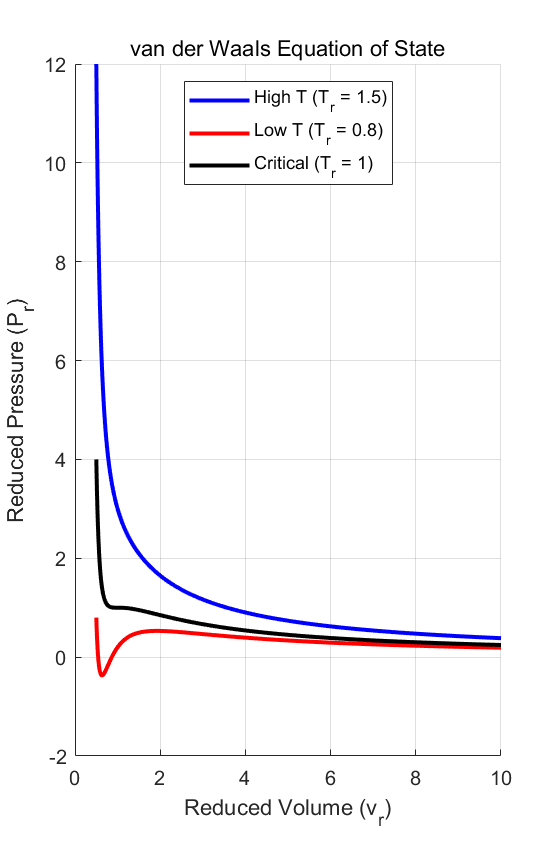
\includegraphics[width=0.4\textwidth,height=0.54\textwidth]{fig/vdw.png}
	\end{figure}
  \end{enumerate}

\subsection{Maxwell Equal Area Construction}

\textbf{Derive for the Maxwell equal area construction.}
  
  The van der Waals equation of state for a non-ideal gas is given by
  \begin{align*}
    P = \frac{RT}{v-b} - \frac{a}{v^{2}}
  \end{align*}
  
  The Maxwell construction replaces an unphysical "loop" with a horizontal line(Constant $P$), reprensenting liquid-vapor coexistence. Conditions for phase equilibrium are:
  \begin{align*}
    P(T,V_{g}) &= P(T,V_{l}) = P_{\text{sat}},\quad V_{g/l}\text{: the molar volume of gas/liquid phases.}\\
    \mu_{g}(T,P) &= \mu_{l}(T,P) 
  \end{align*}
  Since $G = \mu N$ and $\mathrm{d}G = -S\mathrm{d}T + V\mathrm{d}P$, we have:
  \begin{align*}
    \mu_{g} - \mu_{l} = \int_{V_{l}}^{V_{g}}\left(\frac{\partial \mu}{\partial V}\right)_{T}\mathrm{d}V = \int_{V_{l}}^{V_{g}}v\mathrm{d}P = 0
  \end{align*}
  Since $P$ is constant ($P_{\text{sat}}$) along the coexistence line, we can write:
  \begin{align*}
    \int_{V_{l}}^{V_{g}}v\mathrm{d}P = P_{\text{sat}}(V_{g}-V_{l}) - \int_{P_{l}}^{P_{g}}P\mathrm{d}V = 0
  \end{align*}
  And we know that $P_{l} = P_{g} = P_{\text{sat}}$, so this reduces to
  \begin{align*}
    \boxed{\int_{V_{l}}^{V_{g}}P\mathrm{d}V = P_{\text{sat}}(V_{g}-V_{l})},
  \end{align*}
  which is the conclusion to be derived.

  \subsection{Virial Expansion}
  \textbf{Assume that in the virial expansion
  \begin{align*}
    \frac{Pv}{kT} = 1 - \sum_{j=1}^{\infty}\frac{j}{j+1}\beta_{j}\left(\frac{\lambda^{3}}{v}\right)^{j},
  \end{align*}
  where $\beta_{j}$ are the irreducible cluster integrals of the system, only terms with $j = 1$ and $j = 2$ are appreciable in the critical region. }
  \begin{enumerate}
    \item \textbf{Determine the relationship between $\beta_{1}$ and $\beta_{2}$ at the critical point, and} 
    
    Since only the first two terms are appreciable, we can write the virial expansion as:
  \begin{align*}
    \frac{Pv}{kT} \simeq 1 - \left(\frac{1}{2}\beta_{1}\frac{\lambda^{3}}{v} + \frac{2}{3}\beta_{2}\frac{\lambda^{6}}{v^{2}}\right) = 1 - \frac{\beta_{1}\lambda^{3}}{2v} - \frac{2\beta_{2}\lambda^{6}}{3v^{2}}.
  \end{align*}
  Or we can write it as a pressure function $P$ of variable $v$:
  \begin{align*}
    P = kT\left(v^{-1} - \frac{\beta_{1}\lambda^{3}}{2}v^{-2} - \frac{2\beta_{2}\lambda^{6}}{3}v^{-3}\right)
  \end{align*}
  So list the derivatives of $P$ with respect to $v$:
  \begin{align*}
    \frac{\partial P}{\partial v} &= kT(-v^{-2} + \beta_{1}\lambda^{3}v^{-3} + 2\beta_{2}\lambda^{6}v^{-4}) (= 0),\\
    \frac{\partial^{2}P}{\partial v^{2}} &= kT(2v^{-3} - 3\beta_{1}\lambda^{3}v^{-4} - 8\beta_{2}\lambda^{6}v^{-5}) (= 0),
  \end{align*}
  which brings the critical point conditions:
  \begin{align*}
    -v_{c}^{-2} + \beta_{1}\lambda^{3}v_{c}^{-3} + 2\beta_{2}\lambda^{6}v_{c}^{-4} &= 0,\\
    2v_{c}^{-3} - 3\beta_{1}\lambda^{3}v_{c}^{-4} - 8\beta_{2}\lambda^{6}v_{c}^{-5} &= 0.
  \end{align*}
  We can rewrite the equations as
  \begin{align}
    -v_{c}^{2} + \beta_{1}\lambda^{3}v_{c} + 2\beta_{2}\lambda^{6} &= 0,\label{eq:1}\\
    2v_{c}^{2} - 3\beta_{1}\lambda^{3}v_{c} - 8\beta_{2}\lambda^{6} &= 0.\label{eq:2}
  \end{align}
  So the target is to eliminate terms like $v_{c}$. \eqref{eq:1}$\times 2 + $\eqref{eq:2} gives
  \begin{align*}
    (2v_{c}^{2} - 2v_{c}^{2}) &= (3\beta_{1}\lambda^{3}v_{c} - 2\beta_{1}\lambda^{3}v_{c}) + (8\beta_{2}\lambda^{6} - 4\beta_{2}\lambda^{6})\\
    \Rightarrow 0 &= \beta_{1}\lambda^{3}v_{c} + 4\beta_{2}\lambda^{6}\Rightarrow \boxed{\beta_{1} = -\frac{4\beta_{2}\lambda^{3}}{v_{c}}}.
  \end{align*}
  Substitute this into \eqref{eq:1} gives:
  \begin{align*}
    v_{c}^{2} &= \left(-4\beta_{2}\frac{\lambda^{3}}{v_{c}}\right)\lambda^{3}v_{c} + 2\beta_{2}\lambda^{6}\\
    \Rightarrow v_{c}^{2} &= -2\beta_{2}\lambda^{6}\Rightarrow \boxed{v_{c} = \sqrt{-2\beta_{2}}\lambda^{3}}
  \end{align*}
  This connects $\beta_{1}$ and $\beta_{2}$:
  \begin{align*}
    \beta_{1} = -\frac{4\beta_{2}\cancel{\lambda^{3}}}{\sqrt{-2\beta_{2}}\cancel{\lambda^{3}}} = 2\sqrt{-2\beta_{2}}.
  \end{align*}
  So we have $\begin{aligned}
    \boxed{\beta_{1} = 2\sqrt{-2\beta_{2}}}
  \end{aligned}$.

    \item \textbf{show that $\begin{aligned}
      \frac{kT_{c}}{P_{c}v_{c}} = 3
    \end{aligned}$.}

    From the previous problem, we have $\begin{aligned}
      \beta_{1} = \frac{2v_{c}}{\lambda^{3}}
    \end{aligned}$ and $\begin{aligned}
      \beta_{2} = -\frac{v_{c}^{2}}{2\lambda^{6}}
    \end{aligned}$. Substituting these into the virial expansion gives:
    \begin{align*}
      \frac{P_{c}v_{c}}{kT_{c}} &\simeq 1 - \frac{2v_{c}}{\lambda^{3}} \cdot\frac{\lambda^{3}}{2v_{c}} - \left(-\frac{v_{c}^{2}}{2\lambda^{6}}\right)\frac{2\lambda^{6}}{3v_{c}^{2}}\\
      &= 1 - 1 + \frac{1}{3} = \frac{1}{3}
    \end{align*}
    So we have $\begin{aligned}
      \boxed{\frac{kT_{c}}{P_{c}v_{c}} = 3}
    \end{aligned}$
  \end{enumerate}
\end{document}